\chapter{Introducción específica} % Main chapter title

\label{Chapter2}

%----------------------------------------------------------------------------------------
%	2.1 ENFOQUE DEL PROBLEMA
%----------------------------------------------------------------------------------------
ESCRIBIR PARRAFO INTRODUCTORIO

\section{Enfoque del problema}
\label{sec:Enfoque del problema}

El presente trabajo se estructura en torno a tres etapas principales, las cuales se 
encuentran ilustradas en la figura \ref{fig:Etapas de trabajo}.


\begin{figure}[ht]
	\centering
	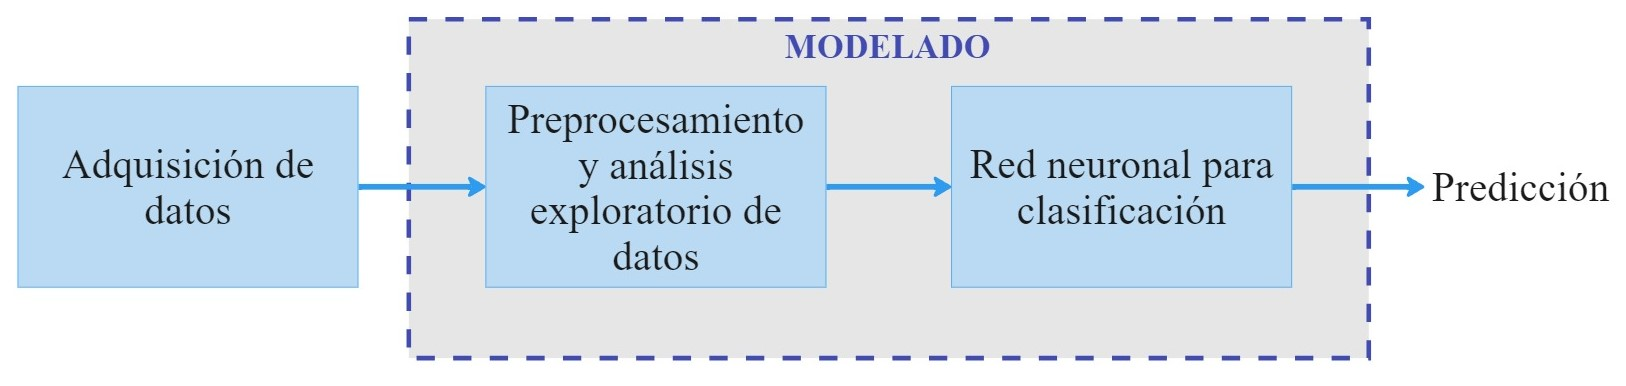
\includegraphics[width=\textwidth]{./Figures/Etapas de trabajo.jpg}
	\caption{Representación esquemática de las etapas del trabajo.}\label{fig:Etapas de trabajo}
\end{figure}

Para comenzar, se llevó a cabo la adquisición de datos. 
Esta etapa fue realizada en colaboración con el servicio de cardiología del Hospital Alemán. 
Para ello, se recopiló información proveniente de presurometrías realizadas a pacientes 
hipertensos a partir del año 2013. Además, se efectuó un análisis exhaustivo de la historia 
clínica de cada paciente con el objetivo de identificar la ocurrencia de eventos cardiovasculares 
adversos mayores. De esta manera, se logró completar el dataset con la variable a predecir (MACE) 
para cada paciente. Asimismo, se enriqueció el conjunto de datos con información clínica adicional 
con el fin de contar con variables explicativas más amplias para abordar el problema de investigación.

A continuación, se efectuó una etapa de preprocesamiento. En primer lugar, se procedió a realizar 
una limpieza de los datos con el propósito de seleccionar las variables más representativas del 
problema. Este proceso de selección permitió eliminar datos redundantes, ruidosos o de poca 
utilidad para el análisis posterior. También, se realizó un análisis exploratorio de datos 
para comprender de manera más profunda las características y patrones presentes en el dataset. 
Esto proporcionó una visión más completa y significativa del conjunto de datos, permitiendo 
así una mejor comprensión de la naturaleza del problema y orientando la toma de decisiones 
posteriores en el desarrollo de este trabajo.

Por último, se procedió al diseñó y entrenamiento de dos modelos de clasificación utilizando 
redes neuronales. El primer modelo se construyó exclusivamente con los datos de presurometrías, 
mientras que el segundo modelo se enriqueció al incluir también los datos clínicos. El propósito 
de esta estrategia fue analizar y comparar el rendimiento de los dos modelos y evaluar si los 
datos de MAPA tienen un sustento suficiente para predecir la variable objetivo MACE. De esta 
manera, se buscó determinar si la inclusión de información clínica adicional contribuyó a 
mejorar las métricas de desempeño en la predicción de MACE, y si podría tener implicancias 
clínicas relevantes para el seguimiento de los pacientes.

%----------------------------------------------------------------------------------------
%	2.2 ALGORITMOS DE CLASIFICACION
%----------------------------------------------------------------------------------------

\section{Algoritmos de clasificación}
\label{sec:Algoritmos de clasificación}

\subsection{Fundamentos y aplicaciones de los modelos de clasificación}

\subsection{Estrategias para tratar el desbalance de clases}

\subsection{Métricas de evaluación en modelos de clasificación}